% Options for packages loaded elsewhere
\PassOptionsToPackage{unicode}{hyperref}
\PassOptionsToPackage{hyphens}{url}
%
\documentclass[
]{book}
\usepackage{amsmath,amssymb}
\usepackage{lmodern}
\usepackage{iftex}
\ifPDFTeX
  \usepackage[T1]{fontenc}
  \usepackage[utf8]{inputenc}
  \usepackage{textcomp} % provide euro and other symbols
\else % if luatex or xetex
  \usepackage{unicode-math}
  \defaultfontfeatures{Scale=MatchLowercase}
  \defaultfontfeatures[\rmfamily]{Ligatures=TeX,Scale=1}
\fi
% Use upquote if available, for straight quotes in verbatim environments
\IfFileExists{upquote.sty}{\usepackage{upquote}}{}
\IfFileExists{microtype.sty}{% use microtype if available
  \usepackage[]{microtype}
  \UseMicrotypeSet[protrusion]{basicmath} % disable protrusion for tt fonts
}{}
\makeatletter
\@ifundefined{KOMAClassName}{% if non-KOMA class
  \IfFileExists{parskip.sty}{%
    \usepackage{parskip}
  }{% else
    \setlength{\parindent}{0pt}
    \setlength{\parskip}{6pt plus 2pt minus 1pt}}
}{% if KOMA class
  \KOMAoptions{parskip=half}}
\makeatother
\usepackage{xcolor}
\IfFileExists{xurl.sty}{\usepackage{xurl}}{} % add URL line breaks if available
\IfFileExists{bookmark.sty}{\usepackage{bookmark}}{\usepackage{hyperref}}
\hypersetup{
  pdftitle={Méthodes numériques},
  pdfauthor={Bruno Duchesne},
  hidelinks,
  pdfcreator={LaTeX via pandoc}}
\urlstyle{same} % disable monospaced font for URLs
\usepackage{longtable,booktabs,array}
\usepackage{calc} % for calculating minipage widths
% Correct order of tables after \paragraph or \subparagraph
\usepackage{etoolbox}
\makeatletter
\patchcmd\longtable{\par}{\if@noskipsec\mbox{}\fi\par}{}{}
\makeatother
% Allow footnotes in longtable head/foot
\IfFileExists{footnotehyper.sty}{\usepackage{footnotehyper}}{\usepackage{footnote}}
\makesavenoteenv{longtable}
\usepackage{graphicx}
\makeatletter
\def\maxwidth{\ifdim\Gin@nat@width>\linewidth\linewidth\else\Gin@nat@width\fi}
\def\maxheight{\ifdim\Gin@nat@height>\textheight\textheight\else\Gin@nat@height\fi}
\makeatother
% Scale images if necessary, so that they will not overflow the page
% margins by default, and it is still possible to overwrite the defaults
% using explicit options in \includegraphics[width, height, ...]{}
\setkeys{Gin}{width=\maxwidth,height=\maxheight,keepaspectratio}
% Set default figure placement to htbp
\makeatletter
\def\fps@figure{htbp}
\makeatother
\setlength{\emergencystretch}{3em} % prevent overfull lines
\providecommand{\tightlist}{%
  \setlength{\itemsep}{0pt}\setlength{\parskip}{0pt}}
\setcounter{secnumdepth}{5}
\usepackage{booktabs}
\usepackage[french]{babel}
\ifLuaTeX
  \usepackage{selnolig}  % disable illegal ligatures
\fi
\usepackage[]{natbib}
\bibliographystyle{plainnat}

\title{Méthodes numériques}
\author{Bruno Duchesne}
\date{2022-04-08}

\usepackage{amsthm}
\newtheorem{theorem}{Théorème}[chapter]
\newtheorem{lemma}{Lemme}[chapter]
\newtheorem{corollary}{Corollaire}[chapter]
\newtheorem{proposition}{Proposition}[chapter]
\newtheorem{conjecture}{Conjecture}[chapter]
\theoremstyle{definition}
\newtheorem{definition}{Définition}[chapter]
\theoremstyle{definition}
\newtheorem{example}{Exemple}[chapter]
\theoremstyle{definition}
\newtheorem{exercise}{Exercice}[chapter]
\theoremstyle{definition}
\newtheorem{hypothesis}{Hypothèse}[chapter]
\theoremstyle{remark}
\newtheorem*{remark}{Remarque}
\newtheorem*{solution}{Solution}
\begin{document}
\maketitle

{
\setcounter{tocdepth}{1}
\tableofcontents
}
\hypertarget{introduction}{%
\chapter*{Introduction}\label{introduction}}
\addcontentsline{toc}{chapter}{Introduction}

Dans ce cours de méthodes numériques, il sera question essentiellement de suites. Celles-ci sont au coeur de l'analyse en mathématiques. Nous donnerons les définitions rigoureuses de limites, continuité et dérivation à l'aide d'\(\varepsilon\) (la lettre grecque epsilon) et \(\delta\) (la lettre grecque delta). Ce sera donc l'occasion d'acquérir les bases de ce domaine des mathématiques alors que vous avez peut-être déjà rencontré les suites et leurs propriétés de manière moins formelle au lycée.

Les suites sont indicées par l'ensemble des entiers naturels \(\mathbb{N}\) et la propriété fondamentale de cet ensemble c'est que chaque entier \(n\in\mathbb{N}\) possède un successeur qui est simplement \(n+1\) et que tous les nombres entiers sont obtenus de cette manière en l'itérant depuis 0 (bref, on obtient tout entier en comptant suffisamment longtemps depuis 0). C'est exactement le \emph{principe de récurrence} qui permet de montrer des propriétés pour des entiers dès lors que l'on peut l'initialiser et justifier l'étape du passage de \(n\) à \(n+1\).

En informatique, c'est la notion de \emph{récursivité} qui joue un rôle analogue. Comprendre les raisonnements par récurrence permet d'appréhender les algorithmes récursifs.

Nous étudierons des suites récurrentes, c'est-à-dire de la forme \(u_{n+1}=f(u_n)\) où \(f\) est unf fonction réelle. Pour pouvoir les étudier, nous aurons besoin de certaines propriétés de la fonction \(f\) comme sa continuité ou sa dérivabilité. Ce sera l'occasion de revenir sur ces points.

Les suites apparaissent aussi de manière cruciale en informatique dans des questions de complexité algorithmique. De manière informelle considérent un algorithme qui prend en entrée des données dont on note \(n\) la taille (par exemple le nombre de bits) et on note \(c_n\) le temps de calcul pour une donnée de taille \(n\). Plus les données sont grandes (\(n\) est grand) plus le temps de calcul est grand. On écrira \(c_n\to+\infty\). La question est de savoir à quelle vitesse la suite \(c_n\) grandit.

En pratique, si la croissance est trop forte (par exemple exponentielle) alors l'algorithme ne s'arretera pas en un temps raisonnable pour des données de grande taille. Ainsi, l'algorithme ne sera pas utile dans ce cas. C'est sur cette impossibilité pratique que reposent certains algorithmes comme le famuex algorithme RSA utilisé en cryptographie.

Les ordinateurs ne manipulent que des données finies (des suites finies de 0 et 1 plus précisément). Comment manipulez des nombres comme \(\sqrt{2}\) ou \(\pi\) qui ne sont pas rationnels et encore moins décimaux ? On fera alors des calculs approchés. Plus précisément, on calculera des approximations d'un tel nombre \(l\), c'est-à-dire des suites \(x_n\) telles que \(x_n\to l\) et on choisira \(n\) suffisamment grand pour obtenir la précision désirée.

\hypertarget{suites}{%
\chapter{Suites}\label{suites}}

\begin{definition}
Une \emph{suite numérique} est la donnée pour tout \(n\in\mathbb{N}\) d'un nombre réel \(x_n\in\mathbb{R}\). On notera alors cette suite \((x_n)_{n\in\mathbb{N}}\) ou simplement \((x_n)\).
\end{definition}

Une suite numérique est donc exactement une application de \(\mathbb{N}\) dans \(\mathbb{R}\). On dit que \(x_n\) est le \emph{terme général} de la suite \((x_n)\).

\begin{example}

Voici quelques exemples de suites.

\begin{enumerate}
\def\labelenumi{\arabic{enumi}.}
\tightlist
\item
  Une suite est \emph{arithmétique} s'il existe un nombre \(r\in\mathbb{R}\) appelé \emph{raison} tel que \(x_{n+1}=x_n+r\) pour tout \(n\in\mathbb{N}\).
\item
  Une suite est \emph{géométrique} s'il existe un nombre \(a\in\mathbb{R}\setminus\{0\}\) tel que \(x_{n+1}=ax_n\) pour tout \(n\in\mathbb{N}\).
\item
  Notons \(m_n\) le nombre de malades du COVID au \(n\)-ième jour depuis le début de l'épidémie alors \((m_n)_{n\in\mathbb{N}}\) est une suite.
\item
  On considère un algorithme de tri de listes. Pour un liste de taille \(n\), on note \(c_n\) le nombre maximal d'opérations à effectuer. Alors \((c_n)\) est une suite.
\end{enumerate}

\end{example}

\hypertarget{monotonie}{%
\section{Monotonie}\label{monotonie}}

\begin{definition}
Soit \(S=(x_n)\) une suite numérique.

On dit que \(S\) est \emph{croissante} si pour tout \(n\leq m\), \(x_n\leq x_m\).

On dit que \(S\) est \emph{décroissante} si pour tout \(n\leq m\), \(x_n\geq x_m\).

Finalement, on dit qu'une suite est \emph{monotone} si elle est croissante ou décroissante.
\end{definition}

\begin{lemma}
Une suite \((x_n)\) est croissante (respectivement décroissante) si et seulement si pour tout \(n\in\mathbb{N}\), \(x_n\leq x_{n+1}\) (respectivement \(x_n\geq x_{n+1}\)).
\end{lemma}

\begin{proof}
La preuve est identique pour les suites croissantes et décroissantes. On ne traite que le cas croissant.

Supposons \((x_n)\) croissante. Alors pour \(n\) fixé, on applique la définition de croissance à \(n\) et \(m=n+1\) et on obtient \(x_n\leq x_{n+1}\).

Réciproquement, on suppose que pour tout \(k\in \mathbb{N}\), \(x_k\leq x_{k+1}\). Fixons \(n,m\in\mathbb{N}\) avec \(n\leq m\). Montrons par récurrence sur \(i\in\mathbb{N}\) que \(x_n\leq x_{n+i}\). Pour \(i=0\), on a bien \(x_n=x_{n+0}\) ce qui initialise la réccurence.

On suppose le résultat pour \(i\). Par hypothèse de récurrence, on a \(x_n\leq x_{n+i}\) et a aussi \(x_{n+i}\leq x_{n+i+1}\) donc \(x_n\leq x_{n+i}\leq x_{n+i+1}\) et donc \(x_n\leq x_{n+i+1}\). Ce qui montre l'étape de récurrence. Par principe de récurrence, nous avons bien \(x_n\leq x_{n+i}\) pour tout \(i\in\mathbb{N}\). On applique le résultat à \(i=m-n\in\mathbb{N}\) et on a donc \(n+i=m\) et donc \(x_n\leq x_m\). Ce que l'on voulait montrer.
\end{proof}

\hypertarget{convergence}{%
\section{Convergence}\label{convergence}}

On rappelle que la \emph{valeur absolue} d'un nombre réel \(x\) est le nombre positif noté \(|x|\) avec \(|x|=x\) si \(x\geq0\) et \(|x|=-x\) si \(x\leq0\). On a toujours l'inégalité \(x\leq|x|\) et \(|-x|=|x|\). On utilisera souvent des inégalités du type \(|x-y|\leq \varepsilon\), ce qui est équivalent à la double inégalité suivante :

\[-\varepsilon\leq x-y\leq \varepsilon.\]

\begin{lemma}[inégalité triangulaire]
Soit \(x,y\in\mathbb{R}\), on a \[|x+y|\leq |x|+|y|.\]
\end{lemma}

\begin{proof}

On sépare en 4 cas selon les signes de \(x\) et \(y\).

\begin{enumerate}
\def\labelenumi{\arabic{enumi}.}
\tightlist
\item
  Si \(x,y\geq0\) alors \(|x+y|=x+y=|x|+|y|\).
\item
  Si \(x,y\leq0\) alors \(|x+y|=|-x-y|\) et on est ramené au cas précédent en considérant \(-x\) et \(-y\) qui sont positifs.
\item
  Si \(x\geq0\) et \(y\leq0\) alors \(x+y\leq x\) et \(-x-y \leq -y=|y|\).
\item
  Si \(x\leq0\) et \(y\geq0\), on se ramène au cas précédent en échangeant les rôles de \(x\) et \(y\).
\end{enumerate}

\end{proof}

\begin{definition}
Une suite \((x_n)\) \emph{converge} vers une limite \(\ell\) si pour tout \(\varepsilon>0\), il existe \(N\in\mathbb{N}\) tel que pour tout \(n\geq N\), \(|x_n-\ell|\leq\varepsilon\). On notera alors \(\lim x_n=\ell\).

Une suite qui converge vers une limite est appelée \emph{suite convergente}.
\end{definition}

\begin{lemma}
Toute suite admet au plus une limite.
\end{lemma}

\begin{proof}
On raisonne par l'absurde. Suppsons que \((x_n)\) admette deux limites \(\ell_1\) et \(\ell_2\) avec \(\ell_1\neq\ell_2\). On applique la définition de limite avec \(\varepsilon=|\ell_1-\ell_2|/3\). Il existe alors \(N_1\) tel que pour tout \(n\geq N_1\) \(|\ell_1-x_n|<\varepsilon\) et \(N_2\) tel que pour tout \(n\geq N_2\) \(|\ell_2-x_n|<\varepsilon\). Posons \(N=\max\{N_1,N_2\}\) alors pour \(n\geq N\), \(|\ell_1-x_n|<\varepsilon\) et \(|\ell_2-x_n|<\varepsilon\). comme \(|\ell_1-\ell_2|=|\ell_1-x_n+x_n-\ell_2|\), on a \(|\ell_1-\ell_2|\leq|\ell_1-x_n|+|x_n-\ell_2|\) par inégalité triangulaire. Ainsi, \(|\ell_1-\ell_2|\|eq2\varepsilon=2/3|\ell_1-\ell_2|\) et comme \(|\ell_1-\ell_2|\neq0\), on obtient la contradiction \(3\leq2\).
\end{proof}

\begin{definition}
Soit \(A\in\mathbb{R}\) et \((x_n)\) une suite, on dit que \(A\) est un \emph{majorant} de \((x_n)\) si \(x_n\leq A\) pour tout \(n\in\mathbb{R}\). Une suite qui possède un majorant est dite \emph{majorée}.

Soit \(A\in\mathbb{R}\) et \((x_n)\) une suite, on dit que \(A\) est un \emph{minorant} de \((x_n)\) si \(x_n\geq A\) pour tout \(n\in\mathbb{R}\). Une suite qui possède un majorant est dite \emph{minorée}.

Une suite est \emph{bornée} si elle est à la fois majorée et minorée.
\end{definition}

\begin{example}
Une suite \((x_n)\) est \emph{constante} s'il existe \(a\in\mathbb{R}\) tel que \(x_n=a\) pour tout \(n\in\mathbb{N}\). Une suite constante est toujours convergente de limite égale à la constante \(a\).
\end{example}

\begin{example}
\protect\hypertarget{exm:harmonique}{}\label{exm:harmonique}La suite \((1/n)_{n\in\mathbb{N}^*}\) converge vers 0.
\end{example}

\begin{proof}
Fixons \(\varepsilon>0\) alors \(1/\varepsilon>0\) et il existe \(N\in\mathbb{N}^*\) tel que \(N\geq 1/\varepsilon\). Maintenant, pour \(n\geq N\), \(0\leq\frac{1}{n}\leq\frac{1}{N}\leq \varepsilon\) et donc \(\left|\frac{1}{n}-0\right|\leq\varepsilon\) et on a bien montré que \(\lim \frac{1}{n}=0\).
\end{proof}

\begin{figure}
\centering
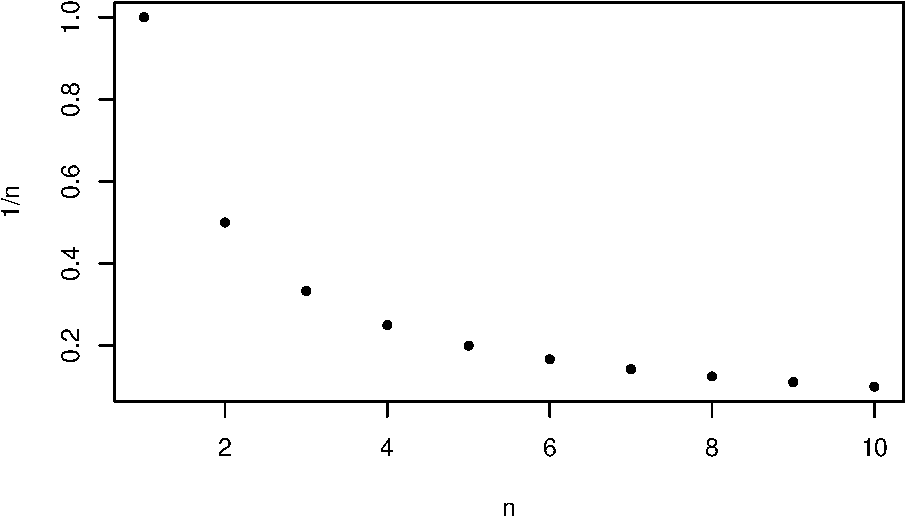
\includegraphics{_main_files/figure-latex/chunk-label-1.pdf}
\caption{\label{fig:chunk-label}Les premières valeurs de la suite de terme général \(x_n=1/n\) qui converge vers 0.}
\end{figure}

\begin{proposition}

Soit \((x_n)\) et \((y_n)\) deux suites convergentes de limites respectives \(\ell_1\) et \(\ell_2\). On a les propriétés suivantes.

\begin{enumerate}
\def\labelenumi{\arabic{enumi}.}
\tightlist
\item
  La suite \(x_n+y_n\) est convergente avec \(\lim x_n+y_n=\ell_1+\ell_2\).
\item
  La suite \(x_ny_n\) est convergente avec \(\lim x_ny_n=\ell_1\ell_2\).
\item
  Si \(\ell_2\neq0\) et \(y_n\neq 0\) pour tout \(n\in\mathbb{N}\) alors la suite \(x_n/y_n\) est convergente avec \(\lim x_n/y_n=\ell_1/\ell_2\).
\item
  Si \(x_n\leq y_n\) pour tout \(n\in\mathbb{N}\) alors \(\ell_1\leq \ell_2\).
\end{enumerate}

\end{proposition}

:::\{.proof\}

\begin{enumerate}
\def\labelenumi{\arabic{enumi}.}
\tightlist
\item
  Soit \(\varepsilon>0\). Comme \(x_n\to\ell_1\), il existe \(N_1\) tel que pour tout \(n\geq N_1\), \(|x_n-\ell_1|\leq \varepsilon/2\). De même, il \(N_1\) tel que pour tout \(n\geq N_2\), \(|x_n-\ell_2|\leq \varepsilon/2\). Maintenant pour \(n\geq\max{N_1,N_2}\), \(|x_n+y_n-(\ell_1-\ell_2)|=|x_n-\ell_1+ y_n-\ell_2|\leq |x_n-\ell_1|+|y_n-\ell_2|\leq \varepsilon/2+\varepsilon/2=\varepsilon\).
\item
\end{enumerate}

\hypertarget{opuxe9rations-sur-les-limites}{%
\section{Opérations sur les limites}\label{opuxe9rations-sur-les-limites}}

\begin{definition}[Bornes supérieures et inférieures]
Si \((x_n)\) est une suite majorée, on note \(\sup x_n\) le plus petit des ses majorants.

Si \((x_n)\) est une suite minorée, on note \(\inf x_n\) le plus petit des ses minorants.
\end{definition}

L'existence des ces bornes supérieures (\(\sup x_n\)) et inférieures (\(\inf x_n\)) n'est pas évidente et une conséquence d'une construction formelle de l'ensemble des nombres réels \(\mathbb{R}\). Nous ne rentrons pas dans ces détails et admettons l'existence des bornes supérieures et inférieures. La construction donne la proposition suivante.

\begin{proposition}
\protect\hypertarget{prp:sup}{}\label{prp:sup}Soit \((x_n)\) une suite majorée (respectivement minorée) de borne supérieure \(A=\sup x_n\) (respectivement borne inférieure \(A=\inf x_n\)) et \(\varepsilon>0\) . Alors il existe \(n\in\mathbb{N}\) tel que \(x_n\geq A-\varepsilon\) (respectivement \(x_n\leq A+\varepsilon\)).
\end{proposition}

\begin{proposition}
Toute suite \((x_n)\) croissante et majorée est convergente vers \(\sup x_n\).
\end{proposition}

\begin{proposition}
Toute suite \((x_n)\) décroissante et minorée est convergente vers \(\inf x_n\).
\end{proposition}

\begin{proof}
La preuve est la même pour les deux proposition en changeant ce qui doit l'être. On prouve seulement la première et on note \(A=\sup x_n\). Soit \(\varepsilon>0\), par la Proposition \ref{prp:sup}, il existe \(n_0\in\mathbb{N}\) tel que \(x_{n_0}\geq A-\varepsilon\).Par croissance, on a aussi \(x_n\geq x_{n_0}\geq A-\varepsilon\) pour \(n\geq n_0\). Comme \(A\) est un majorant, on a aussi \(x_{n}\leq A\) pour tout \(n\in\mathbb{N}\) et donc \(n\in\mathbb{N}\).
\end{proof}

\begin{example}
La suite \((x_n)\) définie par \(x_n=1/n\) pour \(n\in\mathbb{N}^*\) est décroissante et minorée par 0. On a déjà vu qu'elle converge vers 0 dans l'Exemple \ref{exm:harmonique}.
\end{example}

\hypertarget{limites-infinies}{%
\section{Limites infinies}\label{limites-infinies}}

Il existe des cas où une suite ne converge pas mais devient ``aussi grande possible''. La définition suivante rend rigoureuse cette notion.

\begin{definition}
Une suite \((x_n)\) \emph{converge vers \(+\infty\)} si pour tout \(A>0\), il existe \(N\in\mathbb{N}\) tel que pour tout \(n\geq N\), \(x_n\geq A\). On note \(\lim x_n=+\infty\).

Une suite \((x_n)\) \emph{converge vers \(-\infty\)} si pour tout \(A<0\), il existe \(N\in\mathbb{N}\) tel que pour tout \(n\geq N\), \(x_n\leq A\). On note \(\lim x_n=-\infty\).
\end{definition}

\begin{example}
Pour un entier strictement positif \(k\), la suite \((x_n)\) où \(x_n=n^k\) converge vers \(+\infty\).
\end{example}

\begin{proof}
Soit \(A>0\), On choisit \(N\geq A\) et \(N\geq1\), par exemple, \(N=\lfloor A\rfloor+1\) (partie entière plus 1). Pour \(n\geq N\), on a \(n^k=\underbrace{n\times\cdots\times n}_{k\ \textrm{fois}}\geq n\geq N\geq A\) car \(n\geq 1\) et \(k\geq 1\).
\end{proof}

\begin{proposition}
Une suite croissante non majorée converge vers \(+\infty\). De même, une suite décroissante non minorée converge vers \(-\infty\).
\end{proposition}

\begin{proof}
On prouve uniquement le cas d'une suite croissante, la preuve s'adapte pour le cas décroissant. Soit \((x_n)\) une suite croissante non majorée. Soit \(A>0\). Comme la suite n'est pas pas majorée, \(A\) n'est pas un majorant et donc il existe \(n_0\in\mathbb{N}\) tel que \(x_{n_0}>A\) et donc par croissance, pour tout \(n\geq n_0\), \(x_n\geq A\). Ce qui montre bien \(\lim x_n=+\infty\).
\end{proof}

\begin{proposition}

Soit \((x_n)\) et \((y_n)\) avec \(x_n\leq y_n\) pour tout \(n\in\mathbb{N}\).

\begin{itemize}
\tightlist
\item
  Si \(\lim x_n=+\infty\) alors \(\lim y_n=+\infty\).
\item
  Si \(\lim y_n=-\infty\) alors \(\lim x_n=-\infty\).
\end{itemize}

\end{proposition}

\begin{proof}
Supposons \(\lim x_n=+\infty\) et choisissons \(A>0\) alors il existe \(N\in\mathbb{N}\) tel que pour tout \(n\geq N\) \(x_n\geq A\). Ainsi, pour \(n\geq N\), \(y_n\geq x_n\geq A\) et on a prouvé que \(\lim y_n=+\infty\).

Le second cas se traite de manière analogue.
\end{proof}

\hypertarget{deux-exemples}{%
\section{Deux exemples}\label{deux-exemples}}

\hypertarget{suites-arithmuxe9tiques}{%
\subsection{Suites arithmétiques}\label{suites-arithmuxe9tiques}}

\begin{theorem}

Soit \((x_n)\) une suite arithmétique de raison \(r\)

\begin{itemize}
\tightlist
\item
  Si \(r>0\) alors \(\lim x_n=+\infty\).
\item
  Si \(r=0\) alors \(\lim x_n=x_0\).
\item
  Si \(r<0\) alors \(\lim x_n=-\infty\).
\end{itemize}

\end{theorem}

\begin{proof}
Par récurrence, on montre que \(x_n=x_0+nr\).

\begin{itemize}
\tightlist
\item
  Si \(r>0\) alors pour \(A>0\) fixé, on prend \(N=\lfloor (A-x_0)/r\rfloor+1\) et alors pour \(n\geq N\), \(n\geq (A-x_0)/r\), ce qui donne \(x_n=x_0+nr\geq A\) et donc \(\lim x_n=+\infty\).
\item
  Si \(r=0\) alors la suite \((x_n)\) est constante égale à \(x_0\) et converge donc vers cette limite.
\item
  Si \(r<0\) alors pour \(A<0\) fixé, on prend \(N\) entier plus grand que \((A-x_0)/r\) (remarquons que \(A/r>0\) car \(A\) et \(r\) sont négatifs). Maintenant, pour \(n\geq N\), \[n\geq \frac{A-x_0}{r}\] et comme \(r<0\),
\end{itemize}

\[nr\leq A-x_0\]
et donc \(x_n=x_0+nr\leq A\). Ainsi, \(\lim x_n=-\infty\).
\end{proof}

\hypertarget{suites-guxe9omuxe9triques}{%
\subsection{Suites géométriques}\label{suites-guxe9omuxe9triques}}

Commençons avec un petit lemme qui permettra de comparer suite géométrique et arithmétique.

\begin{lemma}[Inégalité de Bernoulli]
Pour tout réel \(a\geq0\) et nombre entier \(n\in\mathbb{N}\), on a

\[(1+a)^n\geq1+na.\]
\end{lemma}

\begin{proof}
On le montre par récurrence sur \(n\). Pour \(n=0\), on obtient \(1=1\) et la récurrence est initialisée. Supposons maintenant le résultat pour \(n\) fixé. Alors \((1+a)^{n+1}=(1+a)^n\cdot(1+a)\geq(1+na)(1+a)=1+(n+1)a+na^2\geq 1+(n+1)a\). Ce qui montre l'étape de récurrence.
\end{proof}

Dans le théorème suivant, on se place dans le cas d'une suite géométrique de premier terme \(x_0\) non nul. En effet, si \(x_0=0\), la suite est constante égale à 0 et il n'y a rien de plus à dire.

\begin{theorem}

Soit \((x_n)\) une suite géométrique de raison \(r\) avec \(x_0\neq0\).

\begin{itemize}
\tightlist
\item
  Si \(r>1\) alors \(\lim x_n=+\infty\) si \(x_0>0\) et \(\lim x_n=-\infty\) si \(x_0<0\).
\item
  Si \(r=1\) alors la suite est constante égale à \(x_0\).
\item
  Si \(|r|<1\) alors \(\lim x_n=0\).
\item
  Si \(r\leq -1\) alors la suite \((x_n)\) n'est pas convergente.
\end{itemize}

\end{theorem}

\begin{proof}

Un raisonnement par récurrence montre que \(x_n= r^nx_0\).

\begin{itemize}
\tightlist
\item
  Si \(r>1\) alors posons \(a=r-1>0\). Ainsi, \(r^n=(1+a)^n\geq 1+na\). Pour \(A>0\), On choisit \(N\) entier supérieur à \(A/a\), ainsi pour \(n\geq N\), \(n\geq A/a\) et donc \$r\^{}n\geq
\item
  Si \(r=1\) alors \(r^n=1\) pour tout \(n\) et donc \(x_n=x_0\) pour tout \(n\).
\item
  Si \(|r|<1\) alros \(1/|r|>1\) et donc par le premier cas, pour tout \(\varepsilon>0\), il existe \(N\in\mathbb{N}\) tel que pour tout \(n\geq N\), \(\left(1/|r|\right)^n\geq \frac{|x_0|}{\varepsilon}\) et ainsi \(|r^nx_0|\leq\varepsilon\). Ce qui montre que \(x_n=r^nx_0\to0\).
\item
  Si \(r< -1\) alors \(|x_n|=|r|^n|x_0|\to\infty\) car \(|r|>1\). Ainsi, la suite n'est pas bornée et donc ne peut pas converger (voir l'Exercice \ref{ex:borne})
\end{itemize}

\end{proof}

\hypertarget{suites-adjacentes}{%
\section{Suites adjacentes}\label{suites-adjacentes}}

\begin{definition}
Soit \((x_n)\) et \((y_n)\) deux suites numériques. On dit que ces suites sont \emph{adjacentes} si \(x_n\geq y_n\) pour tout \(n\in\mathbb{N}\), \((x_n)\) est croissante, \((y_n)\) est décroissante et \(\lim y_n-x_n=0\).
\end{definition}

\begin{proposition}
Si \((x_n)\) et \((y_n)\) sont deux suites adjacentes alors ces deux suites sont convergentes et \(\lim x_n=\lim y_n\).
\end{proposition}

\begin{proof}
La suite \((x_n)\) est croissante majorée (par \(y_0\) par exemple) et donc converge vers une limite \(\ell_1\). De même, \((y_n)\) est décroissante minorée et donc converge vers une limite \(\ell_2\). Ainsi la suite \((y_n-x_n)\) est convergente de limite \(\ell_2-\ell_1\). Comme \(\lim y_n-x_n=0\), on a \(\ell_2-\ell_1=0\) et donc \(\ell_1=\ell_2\).
\end{proof}

\begin{figure}
\centering
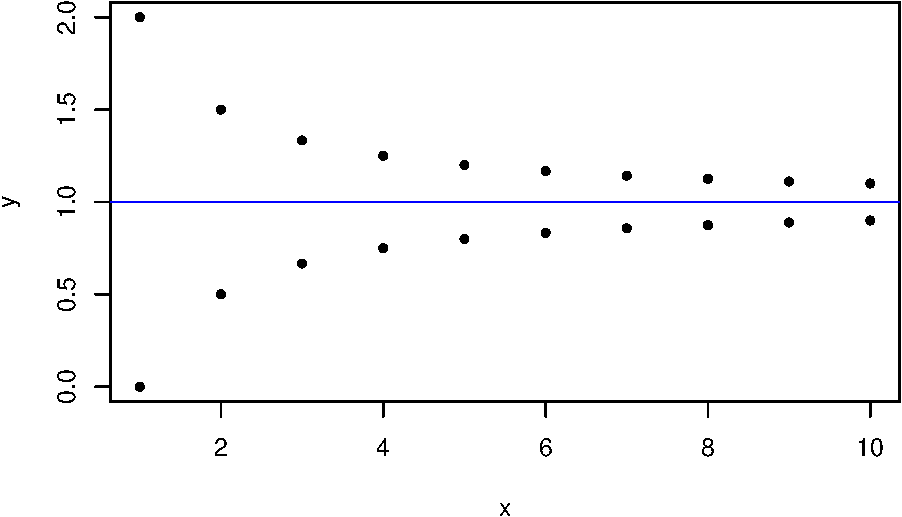
\includegraphics{_main_files/figure-latex/chunk-label-1-1.pdf}
\caption{\label{fig:chunk-label-1}Deux suites adjacentes qui converge vers 1.}
\end{figure}

\begin{theorem}[Théorème des gendarmes]
Soit \((x_n), (y_n)\) et \((u_n)\) trois suites telles que pour tout \(n\in\mathbb{N}\), \(x_n\leq u_n\leq y_n\) et telles \((x_n), (y_n)\) sont convergentes avec \(\lim x_n=\lim y_n=\ell\) alors \((u_n)\) est convergente de limite \(\ell\).
\end{theorem}

\hypertarget{exercices}{%
\section{Exercices}\label{exercices}}

\begin{exercise}
Donner un exemple d'une suite qui n'est pas monotone.
\end{exercise}

\begin{exercise}
Montrer qu'une suite \((x_n)\) est bornée si et seulement s'il existe \(A\geq 0\) tel que pour tout \(n\in \mathbb{N}\), \(|x_n|\leq A\).
\end{exercise}

\begin{exercise}
\protect\hypertarget{exr:borne}{}\label{exr:borne}Montrer qu'une suite convergente est toujours bornée.
\end{exercise}

\begin{exercise}
On définit deux suites \((x_n)\) et \((y_n)\) par \(x_n=2^n\) et \(y_n=3^n\). Déterminer la comportement des suites de termes généraux \(z_n=x_n+y_n\), \(u_n=x_n-y_n\), \(v_n=x_ny_n\), \(w_n=x_n/y_n\) et \(t_n=y_n/x_n\).
\end{exercise}

\begin{exercise}
Soit \((x_n)\) une suite convergente de limite \(\ell\). On pose \(y_n=x_{2n}\) pour tout \(n\in\mathbb{N}\). Montrer que la suite \((y_n)\) est convergente de limite \(\ell\).
\end{exercise}

\begin{exercise}

Soit \(a,b\in \mathbb{R}\). On fixe \(x_0\) et on définit récursivement \(x_{n+1}=ax_n+b\).

\begin{enumerate}
\def\labelenumi{\arabic{enumi}.}
\tightlist
\item
  Déterminer le comportement de \((x_n)\) si \(a=0\) ou \(a=1\).
\item
  On suppose \(a\neq0\). On pose \(c=\frac{b}{a-1}\) et \(y_n=x_n+c\). Montrer que \((y_n)\) est une suite géométrique de raison \(a\).
\item
  En fonction de \(a\), déterminer le comportement de \(y_n\) puis celui de \(x_n\).
\item
  À l'aide de la formule explicite d'une suite géométrique, déduire une formule explicite pour \(x_n\).
\end{enumerate}

\end{exercise}

\hypertarget{continuituxe9-et-duxe9rivation-de-fonctions-ruxe9elles}{%
\chapter{Continuité et dérivation de fonctions réelles}\label{continuituxe9-et-duxe9rivation-de-fonctions-ruxe9elles}}

\hypertarget{continuituxe9}{%
\section{Continuité}\label{continuituxe9}}

\hypertarget{duxe9rivation}{%
\section{Dérivation}\label{duxe9rivation}}

\hypertarget{exponentielle-et-logarithme}{%
\section{Exponentielle et logarithme}\label{exponentielle-et-logarithme}}

\hypertarget{suites-ruxe9currentes}{%
\chapter{Suites récurrentes}\label{suites-ruxe9currentes}}

\hypertarget{approximations}{%
\chapter{Approximations}\label{approximations}}

\hypertarget{notations-de-landau-et-type-de-complexituxe9}{%
\chapter{Notations de Landau et type de complexité}\label{notations-de-landau-et-type-de-complexituxe9}}

\hypertarget{notations-de-landau}{%
\section{Notations de Landau}\label{notations-de-landau}}

\hypertarget{comparaisons-usuelles}{%
\section{Comparaisons usuelles}\label{comparaisons-usuelles}}

\hypertarget{application-uxe0-la-complexituxe9-de-quelques-algorithmes}{%
\section{Application à la complexité de quelques algorithmes}\label{application-uxe0-la-complexituxe9-de-quelques-algorithmes}}

  \bibliography{book.bib,packages.bib}

\end{document}
